\section{Fundamentos de arquitectura de software}

\subsection{Definición de arquitectura de software}
La arquitectura de software es el conjunto de decisiones fundamentales que definen la estructura, organización y comportamiento de un sistema. Al utilizar patrones y principios de diseño, establece un marco de referencia para la construcción, evolución y mantenimiento del software. 

Más allá de organizar componentes, la arquitectura determina cómo se gestionan las interacciones para cumplir con los atributos de calidad (escalabilidad, seguridad, desempeño) y los requerimientos funcionales y no funcionales. Constituye el puente entre los objetivos organizacionales y las soluciones tecnológicas, siendo esencial para garantizar la integridad y viabilidad del sistema \cite{27}.

\subsection{Importancia en el Desarrollo de Sistemas}

La arquitectura es el cimiento técnico que asegura la correcta construcción del sistema adecuado para el negocio, destacando por:

\begin{itemize}
\item \textbf{Gestión de la Complejidad:} Coordina procesos y dependencias mediante flexibilidad y adaptación, controlando factores desconocidos o cambios no anticipados.
\item \textbf{Mitigación de Riesgos Tempranos:} Permite un enfoque proactivo para detectar y neutralizar vulnerabilidades antes de que afecten la operación.
\item \textbf{Escalabilidad:} Garantiza la adaptación del sistema ante variaciones en la carga de trabajo sin afectar su rendimiento ni requerir reingeniería.
\item \textbf{Mantenibilidad:} Facilita modificaciones, correcciones y mejoras futuras gracias a un diseño organizado y claro.
\item \textbf{Toma de Decisiones:} Establece el marco para la elección de tecnologías y la gestión de compromisos técnicos (\textit{trade-offs}).
\end{itemize}

\subsection{Factores de calidad}

Basados en modelos internacionales (ISO/IEC 25010), los atributos de calidad evalúan y garantizan la viabilidad a largo plazo de la arquitectura elegida \cite{28}. En un sistema de gestión de denuncias, destacan:

\begin{itemize}
\item \textbf{Rendimiento y Eficiencia:} Optimización de recursos y latencias mínimas en la comunicación entre microservicios, asegurando una experiencia fluida al cargar evidencias \cite{28}.
\item \textbf{Mantenibilidad:} Facilidad para actualizar o corregir el sistema. El uso de \textit{Docker} y el patrón de tres capas permite modificar microservicios independientemente sin afectar la estabilidad \cite{28}.
\item \textbf{Escalabilidad:} Capacidad de escalar horizontalmente servicios críticos ante altas demandas de usuarios, optimizando la infraestructura institucional \cite{29}.
\item \textbf{Seguridad y Confidencialidad:} Protección de la identidad del denunciante e integridad del expediente mediante cifrado de datos y control de acceso (RBAC).
\item \textbf{Disponibilidad y Tolerancia a Fallos:} Aislamiento de errores entre servicios (ej. la caída del módulo analítico no afecta el sistema central), previniendo el colapso total.
\end{itemize}

Estos factores aseguran que la plataforma sea una herramienta robusta, confiable y duradera para la Defensoría.

\section{Arquitectura del Sistema}

\subsection{Visión general de la arquitectura híbrida}

Para el desarrollo de la “Plataforma Web para la Denuncia Segura y Prevención de Riesgos Digitales”, se ha seleccionado una arquitectura de microservicios, la cual se complementa internamente con un patrón de tres capas para la organización de cada servicio. Esta decisión técnica no es arbitraria; se fundamenta en la necesidad de superar las limitaciones de las arquitecturas monolíticas tradicionales, donde el alto acoplamiento entre componentes suele derivar en dificultades para el mantenimiento y la escalabilidad ante una demanda creciente \cite{30}.

Al adoptar un enfoque de microservicios, el sistema se descompone en unidades funcionales autónomas que se comunican a través de protocolos ligeros. Según Villamizar et al., esta estructura permite que cada componente evolucione de manera independiente, facilitando la innovación tecnológica y permitiendo que fallos en un servicio específico (como el procesador de lenguaje natural en Python) no comprometan la disponibilidad global de la plataforma administrativa en Java \cite{31}.

\subsection{Arquitectura de Microservicios}

La arquitectura de microservicios se define como un enfoque de desarrollo de software donde una aplicación se descompone en un conjunto de servicios pequeños, autónomos y altamente cohesivos. Cada uno de estos componentes se ejecuta como un proceso independiente y se comunica con los demás a través de mecanismos ligeros, generalmente interfaces de programación de aplicaciones (APIs) basadas en el protocolo HTTP.

\begin{figure}[H]
    \centering
    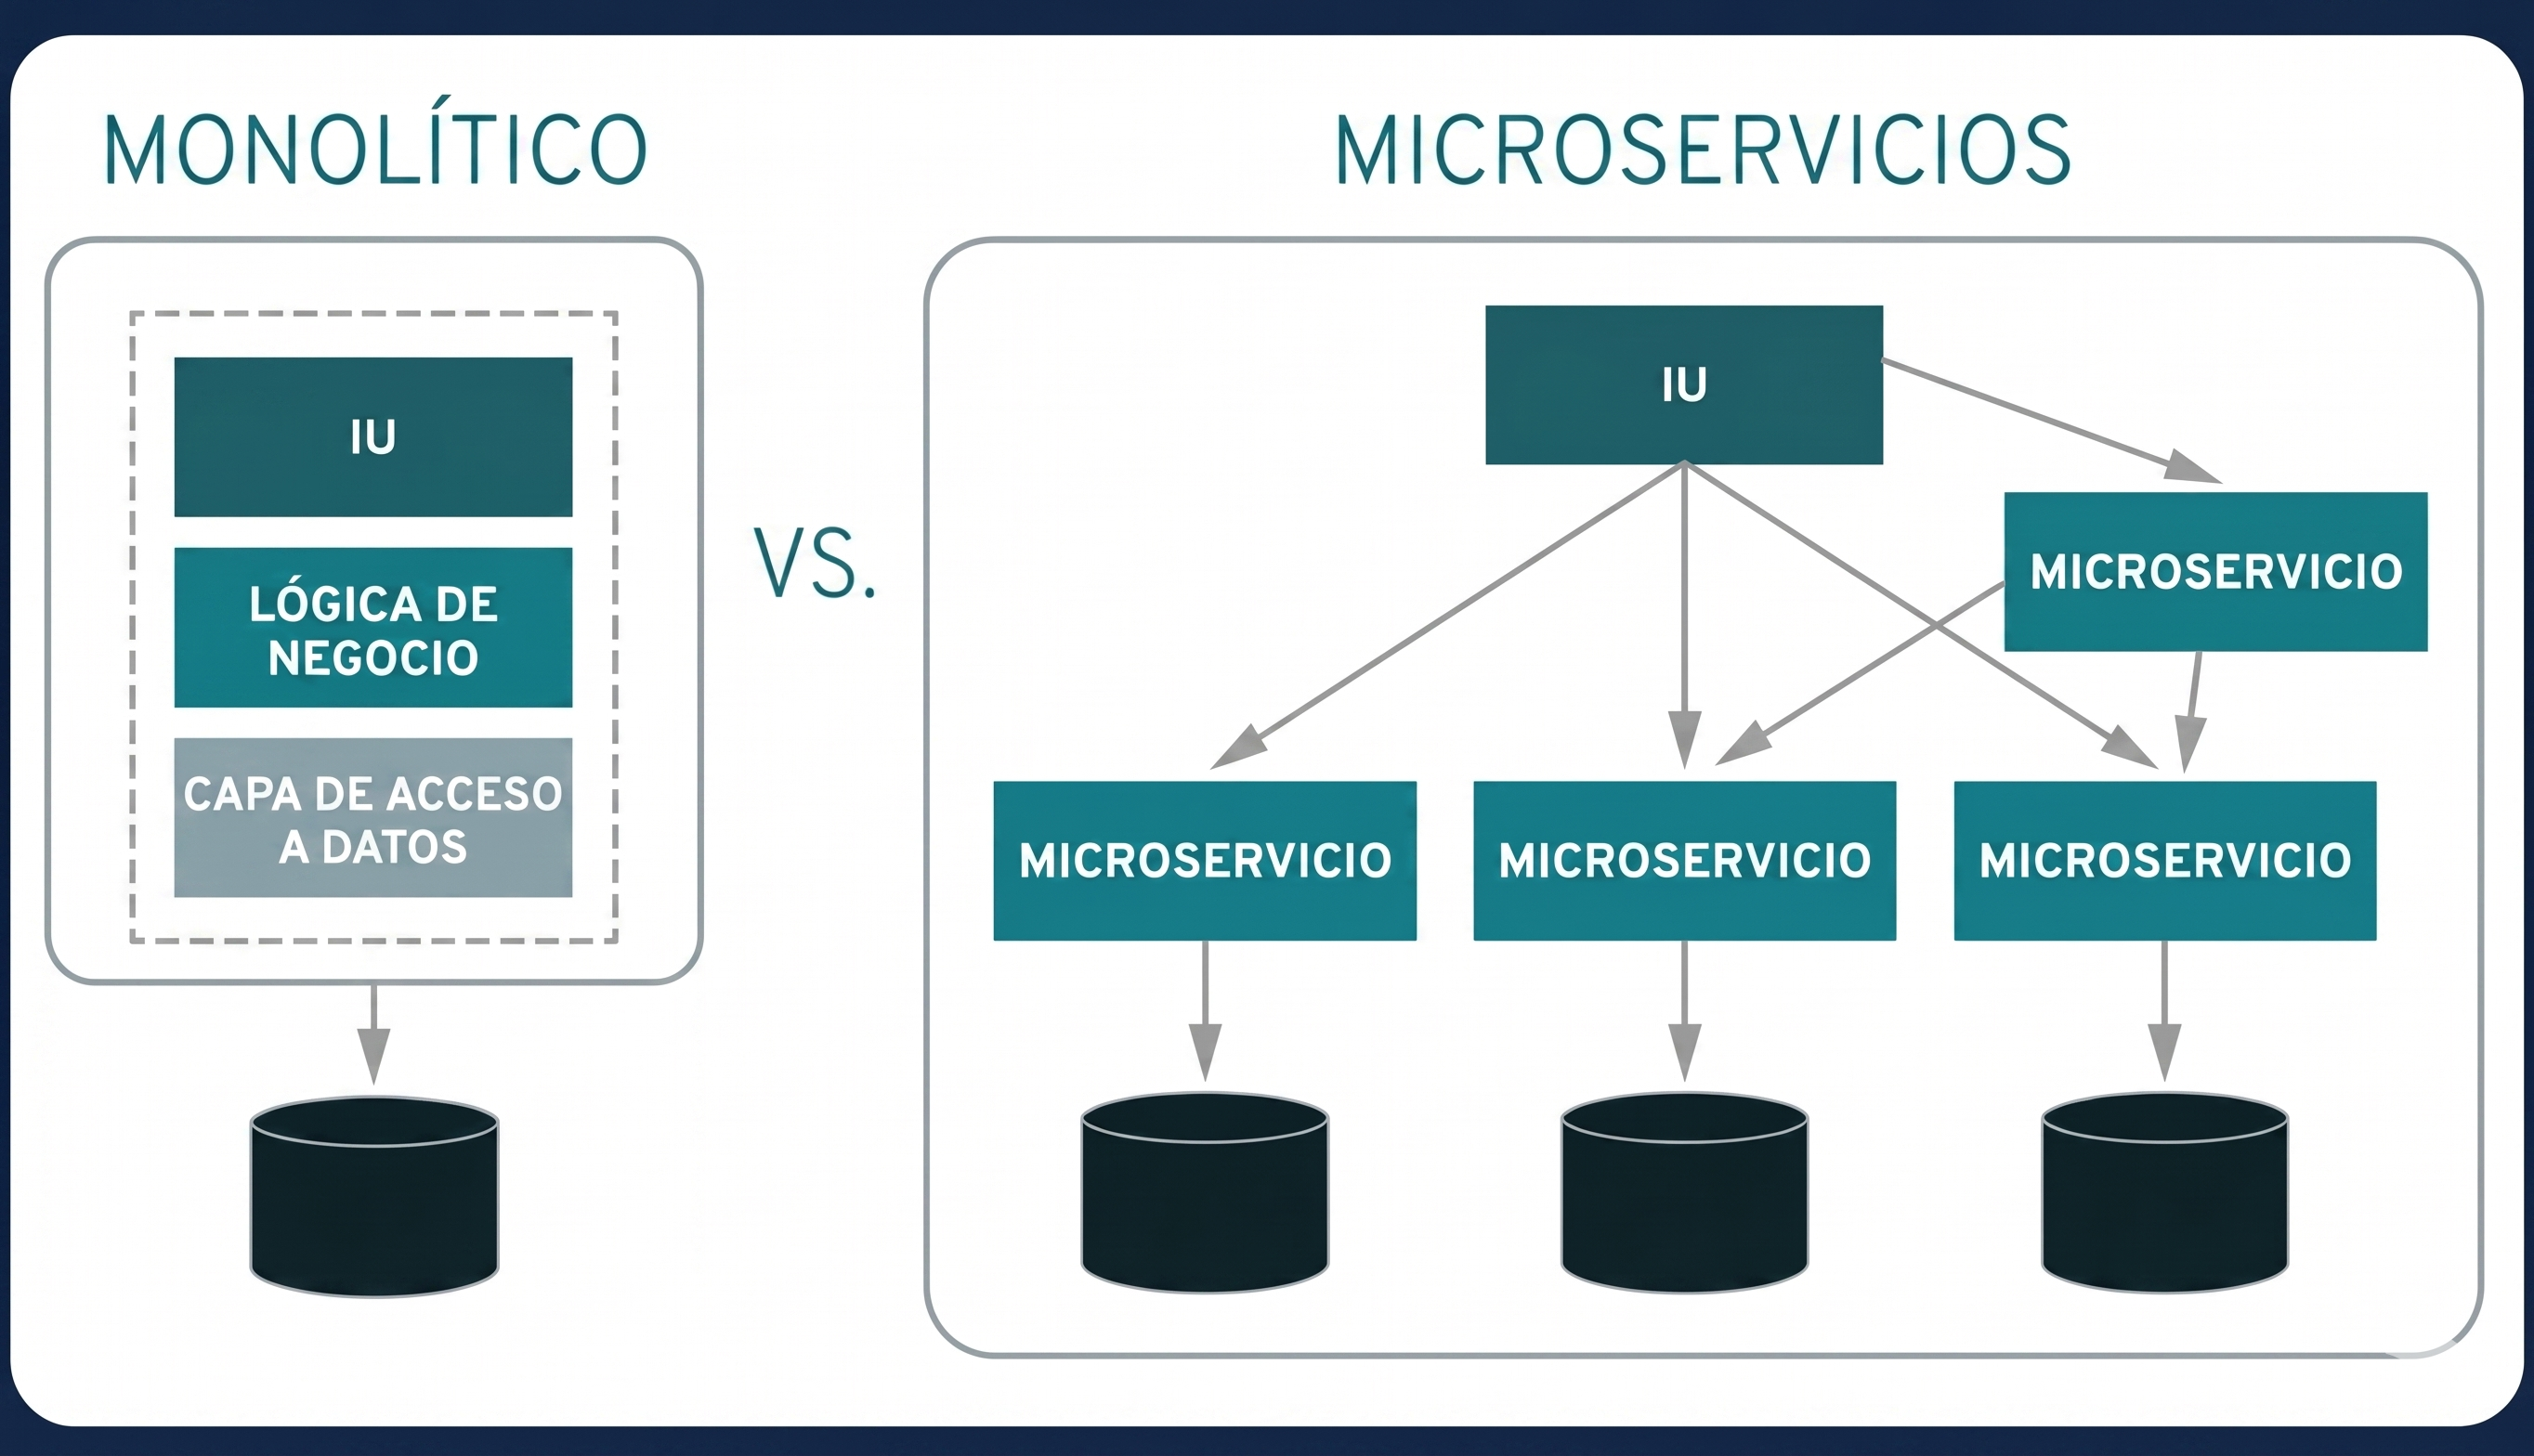
\includegraphics[width=0.7\textwidth]{imagenes/documento/arquitecturademicroservicios.png}
    \caption{Comunicación entre microservicios.}
    \label{fig:microservicios}
\end{figure}

A diferencia de las arquitecturas monolíticas, donde una falla en un módulo puede comprometer la totalidad del sistema, los microservicios permiten que cada unidad funcional se enfoque en una capacidad específica del negocio, facilitando su desarrollo, despliegue y escalado de forma totalmente autónoma \cite{31}.
\textbf{Ventajas de su uso:}
\begin{itemize}
\item \textbf{Aislamiento y Resiliencia ante Fallos:} Dado que cada servicio opera en un entorno de ejecución separado, un error crítico o una excepción no controlada en un módulo específico no provoca un efecto dominó sobre el resto de la plataforma. Esta característica es vital para mantener la alta disponibilidad requerida en entornos institucionales \cite{32}.

\item \textbf{Escalabilidad Granular y Eficiente:} Permite realizar un escalado horizontal selectivo. En lugar de replicar la aplicación completa, es posible asignar recursos de infraestructura adicionales únicamente a aquellos servicios que experimentan una alta demanda de procesamiento, optimizando significativamente el uso del hardware y los costos operativos \cite{32} \cite{29}.

\item \textbf{Heterogeneidad Tecnológica:} Facilita el uso de diferentes lenguajes de programación y bases de datos según las necesidades específicas de cada módulo. En este proyecto, dicha flexibilidad permite la coexistencia de servicios robustos en Java con módulos especializados en análisis de datos desarrollados en Python \cite{32}.

\item \textbf{Agilidad en el Despliegue Continuo:} Al reducir el acoplamiento entre funciones, se acortan los ciclos de desarrollo y se permite la actualización constante de módulos individuales sin necesidad de reiniciar o interrumpir la operación global del sistema \cite{33}.
\end{itemize}

\textbf{Justificación para la Defensoría de los Derechos Politécnicos:}
La elección de este enfoque para la plataforma de denuncia segura responde a la complejidad intrínseca de los procesos administrativos y legales del Instituto. El sistema requiere gestionar múltiples roles y flujos de trabajo (denunciantes, abogados, administradores) que poseen demandas computacionales distintas. Se adoptó esta arquitectura para asegurar la continuidad operativa: si el microservicio encargado del procesamiento de lenguaje natural llegara a saturarse, los módulos de registro de quejas y gestión de expedientes continuarían funcionando de forma ininterrumpida.

\subsection{Arquitectura interna de los servicios: Patrón de 3 capas}

La arquitectura de tres niveles (o capas) es un modelo de diseño de software cuya finalidad primordial es la separación de las responsabilidades y el desacoplamiento de las etapas de procesamiento de una aplicación. Esta estructura organiza el software en tres niveles lógicos y físicos claramente diferenciados: el nivel de presentación, el nivel de aplicación (o lógica de negocio) y el nivel de datos \cite{33} \cite{40}.

\begin{figure}[H]
    \centering
    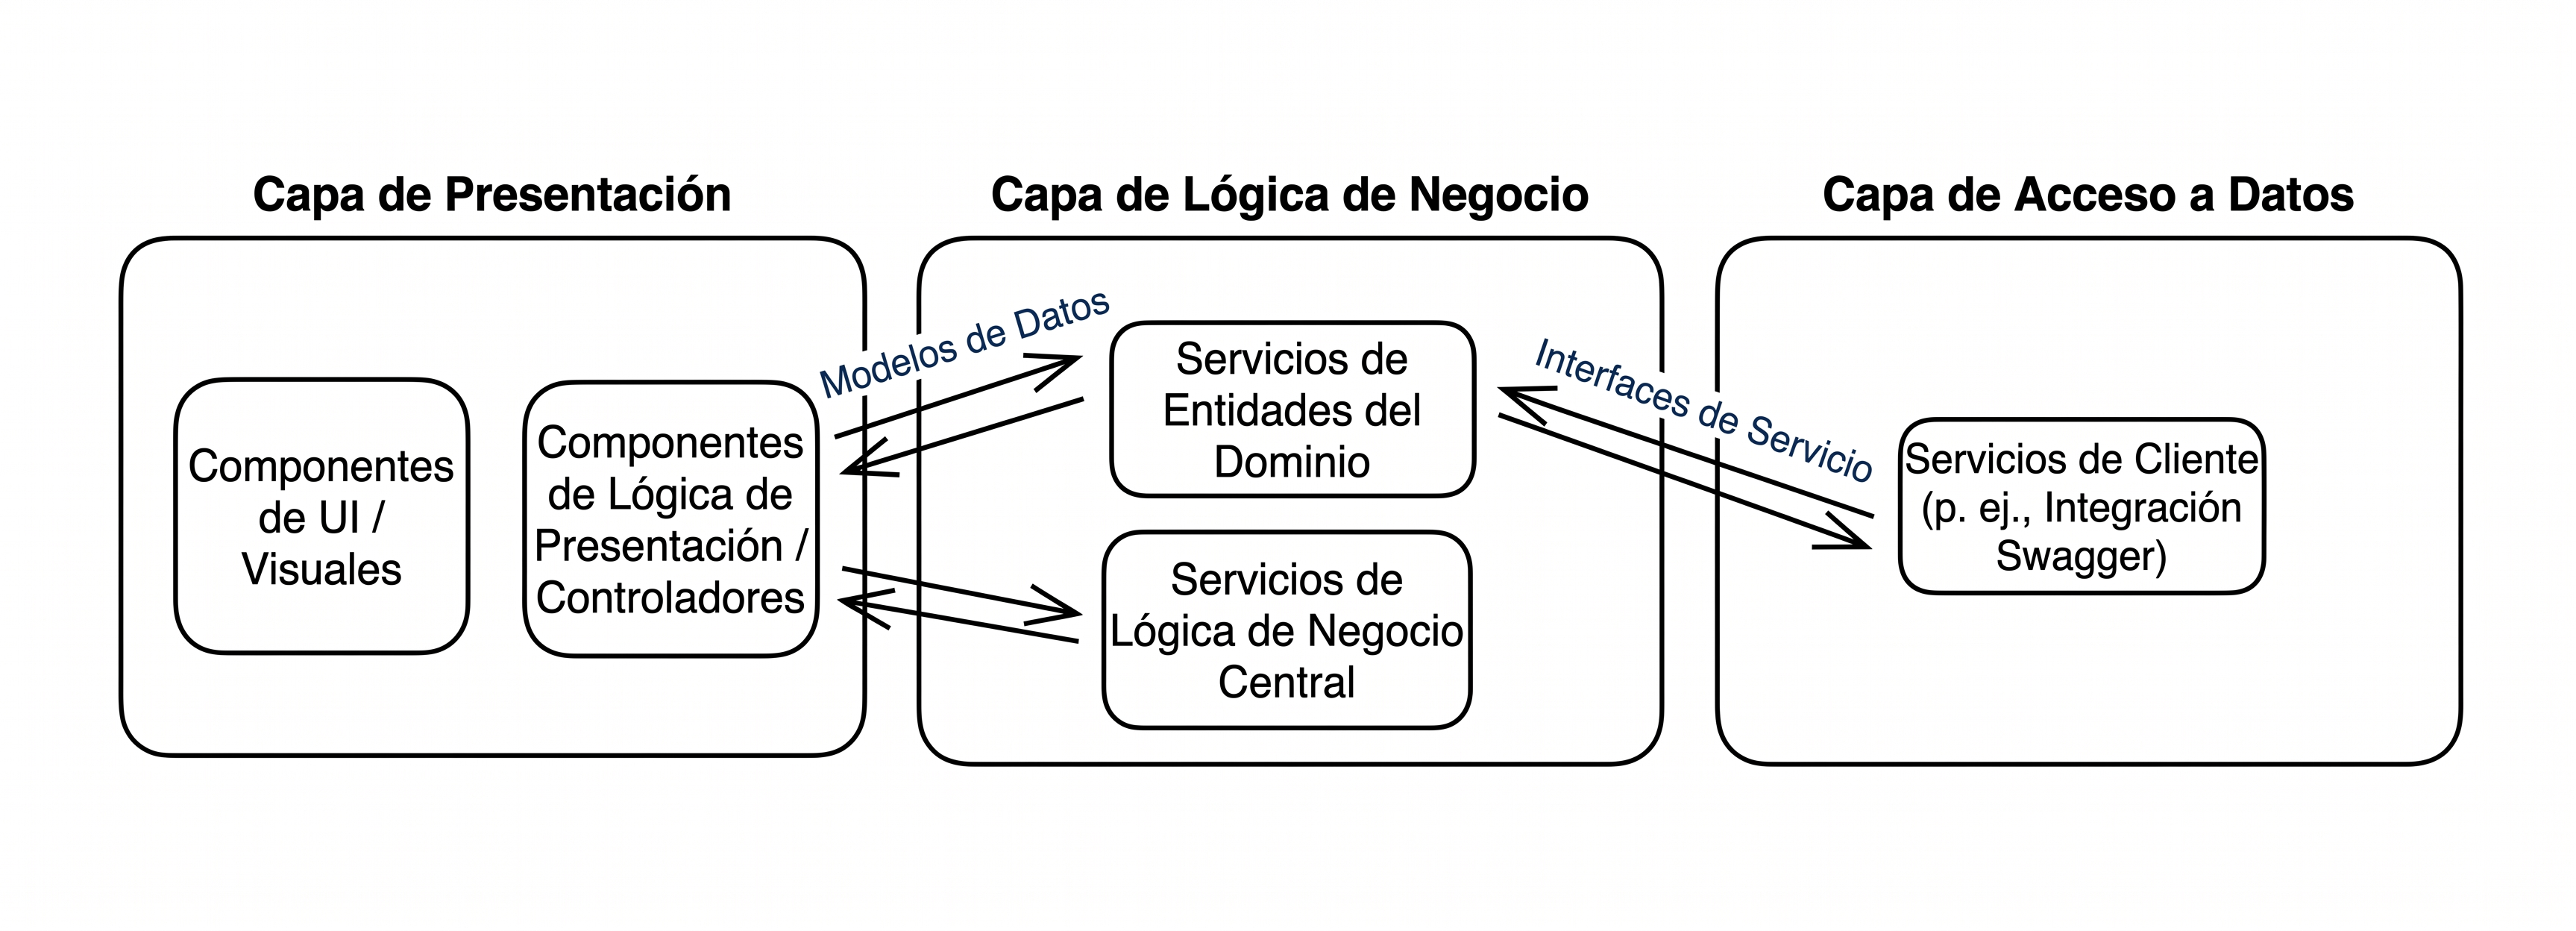
\includegraphics[width=0.7\textwidth]{imagenes/documento/patron3capas.png}
    \caption{Patron de Diseño de 3 capas.}
    \label{fig:patron de diseno de 3 capas}
\end{figure}

En este proyecto, dicha estructura conforma de manera exacta el diseño interno de cada microservicio, garantizando que la lógica institucional esté aislada de las interfaces de usuario y de los motores de persistencia.

\begin{itemize}
\item \textbf{Nivel de Presentación (Interfaz de Usuario):} Es la capa más externa del servicio, encargada de la interacción directa con el usuario o con otros servicios externos. Su función principal es presentar la información y recolectar datos de entrada para enviarlos a la capa de aplicación. Al estar desacoplada, permite realizar cambios estéticos o funcionales en la interfaz (Angular) sin alterar las reglas de negocio subyacentes \cite{33} \cite{40}.

\item \textbf{Nivel de Aplicación (Lógica de Negocio):} Considerado el núcleo del servicio, es donde se modelan las reglas del negocio y se toman las decisiones lógicas. Según Coti Colop, la ubicación de las reglas en esta capa central es crítica para asegurar la funcionalidad y la integridad del sistema, ya que actúa como un puente que coordina las peticiones de la interfaz y la gestión de los datos, protegiendo la coherencia de los procesos legales y administrativos de la Defensoría \cite{33}.

\item \textbf{Nivel de Datos (Persistencia):} Es la capa responsable del almacenamiento y la recuperación de la información. Gestiona la comunicación con el Sistema de Gestión de Bases de Datos (PostgreSQL), permitiendo que la persistencia sea transparente para las capas superiores. Esto significa que el motor de base de datos podría ser optimizado o sustituido con un impacto mínimo en la lógica de negocio \cite{42}.
\end{itemize}

\textbf{Ventajas de su uso:}
\begin{itemize}
\item \textbf{Independencia y Escalabilidad:} Cada nivel puede ser escalado de forma independiente según la demanda específica. Por ejemplo, si el procesamiento de datos aumenta, se puede fortalecer la capa de aplicación sin necesidad de modificar la interfaz de usuario \cite{33} \cite{42}.
\item \textbf{Mantenibilidad y Flexibilidad:} Facilita el mantenimiento a largo plazo al permitir que cada capa sea desarrollada, probada y actualizada simultáneamente por distintos integrantes del equipo, lo que reduce significativamente el tiempo total de desarrollo y el riesgo de introducir errores colaterales \cite{46}.
\item \textbf{Confiabilidad Operativa:} Al operar de manera aislada, una interrupción o fallo en la capa de presentación no compromete la integridad de los datos ni la ejecución de los procesos de negocio en curso, aumentando la resiliencia del microservicio \cite{46}.
\end{itemize}

\subsection{Servidor web y proxy inverso (Nginx)}

NGINX es una infraestructura de software de código abierto diseñada para el servicio de contenido web, el funcionamiento como proxy inverso y la gestión de balanceo de carga. A diferencia de los servidores tradicionales basados en hilos, NGINX destaca por su arquitectura asíncrona basada en eventos, la cual permite gestionar un alto volumen de conexiones concurrentes con una utilización mínima de memoria y CPU.

En el ecosistema de este proyecto, NGINX actúa como el punto de entrada unificado, gestionando el flujo de datos entre el cliente y los servicios internos.

\textbf{Ventajas de su uso:}
\begin{itemize}
\item \textbf{Rendimiento y Manejo de Concurrencia:} Gracias a su arquitectura no bloqueante, el servidor puede procesar miles de peticiones simultáneas sin los costos asociados a la creación de nuevos procesos por cada conexión.

\item \textbf{Balanceo de Carga Eficiente:} Como proxy inverso, NGINX distribuye de manera inteligente las peticiones entrantes entre las distintas instancias de los microservicios.

\item \textbf{Caché y Optimización de Contenido:} Posee la capacidad de almacenar temporalmente contenido estático y respuestas frecuentes, reduciendo el tiempo de respuesta percibido.

\item \textbf{Terminación de SSL/TLS:} NGINX permite centralizar la gestión de certificados de seguridad y el cifrado de las comunicaciones en un solo punto.
\end{itemize}

\textbf{Implementación como API Gateway:}
Dentro de una arquitectura de microservicios, exponer cada módulo directamente a la red pública representaría una vulnerabilidad crítica. En este proyecto, NGINX se implementa bajo el patrón de \textit{API Gateway} (puerta de enlace), interceptando todas las peticiones y enrutándolas mediante reglas de despacho hacia el microservicio interno correspondiente.

\section{Tecnologías de Desarrollo Backend}

\subsection{Lenguaje de programación: Java}

Java es un lenguaje de programación de propósito general, orientado a objetos y una plataforma informática de amplia adopción en el ámbito empresarial. Se destaca históricamente por su portabilidad, seguridad y fiabilidad, siendo una de las tecnologías preferidas para el desarrollo de sistemas distribuidos y aplicaciones de misión crítica.

\subsubsection{Seguridad y tipado estricto}
La seguridad en Java no es una capa superficial, sino una característica intrínseca de su diseño. Se basa en el modelo de \textit{Sandbox} (Caja de Arena), que restringe la ejecución de código no confiable. Java implementa un sistema de tipado fuerte que detecta errores en tiempo de compilación, lo que reduce drásticamente las vulnerabilidades comunes.

\subsubsection{Arquitectura de la Java Virtual Machine (JVM)}
La JVM es el corazón técnico que permite la independencia de plataforma mediante una capa de abstracción entre el código fuente y el hardware. La compilación JIT (Just-In-Time) analiza las secciones de código que se ejecutan con mayor frecuencia y las traduce directamente a código máquina optimizado.

\subsubsection{Gestión de memoria: Garbage Collection (GC)}
A diferencia de lenguajes como C++, Java gestiona la memoria de forma automática, eliminando el riesgo de fugas de memoria. El recolector de basura divide la memoria \textit{Heap} en regiones: \textit{Young Generation} y \textit{Old Generation}, utilizando el algoritmo Mark-and-Sweep.

\subsubsection{Multihilo y concurrencia}
Para manejar múltiples denuncias simultáneas, Java utiliza un modelo de hilos nativos gestionados por el sistema operativo pero controlados por la JVM. Spring Boot utiliza \textit{Thread Pools} que mantienen un número N de hilos activos listos para procesar tareas de una cola de espera.

\subsection{Framework: Spring Boot}

Spring Boot es una extensión del ecosistema Spring diseñada para simplificar el proceso de configuración y despliegue de aplicaciones de grado empresarial. Se basa en el principio de \textit{“Convention over Configuration”} (convención sobre configuración), lo que permite crear microservicios autónomos y listos para producción con un esfuerzo de configuración mínimo \cite{38}.

\subsubsection{Pilares fundamentales}
\begin{itemize}
    \item \textbf{Configuración Automática:} El framework analiza las dependencias presentes en el \textit{classpath} y configura automáticamente los componentes.
    \item \textbf{Spring Starters:} Paquetes de dependencias predefinidos que agrupan todas las librerías necesarias para una funcionalidad específica.
    \item \textbf{Aplicaciones Standalone:} Integra servidores embebidos (Tomcat, Jetty, Undertow) generando un archivo JAR ejecutable.
\end{itemize}

\subsubsection{Inversión de Control (IoC) e Inyección de Dependencias}
El núcleo de Spring Boot se basa en el contenedor de Inversión de Control (IoC) y el patrón de Inyección de Dependencias (DI). Spring gestiona el ciclo de vida de los objetos (\textit{Beans}) e inyecta las dependencias necesarias en tiempo de ejecución.

\subsubsection{Spring Boot Actuator}

Spring Boot Actuator es un subproyecto del ecosistema Spring que proporciona funcionalidades críticas para la \textit{observabilidad} y el monitoreo de aplicaciones en entornos de producción. Según \cite{51}, esta herramienta permite obtener información detallada sobre el estado de ejecución de los componentes internos de la aplicación sin necesidad de implementar código adicional para la recolección de métricas.


Una vez habilitado, el framework expone una serie de puntos de acceso o \textit{endpoints} bajo la ruta base \texttt{/actuator}. Por defecto, y por razones de seguridad, solo el \textit{endpoint} de salud (\texttt{/health}) se encuentra activo, devolviendo un estado simplificado como \texttt{\{"status":"UP"\}} para confirmar que la aplicación está operativa.

\paragraph{Endpoints Principales y Gestión de Beans}
Para un monitoreo exhaustivo, es posible habilitar la exposición de otros puntos de acceso mediante la propiedad \texttt{management.endpoints.web.exposure.include} en el archivo de configuración. Los \textit{endpoints} más relevantes incluyen:

\begin{itemize}
    \item \textbf{/health:} Informa sobre el estado de la aplicación y sus dependencias.
    \item \textbf{/metrics:} Expone métricas de rendimiento como el uso de memoria JVM y CPU.
    \item \textbf{/loggers:} Permite visualizar y modificar los niveles de log en tiempo de ejecución.
    \item \textbf{/beans:} Muestra una estructura JSON detallada de todos los \textit{Spring Beans} registrados.
\end{itemize}

% --- ESPACIO PARA LA IMAGEN ---
\begin{figure}[htbp]
    \centering
    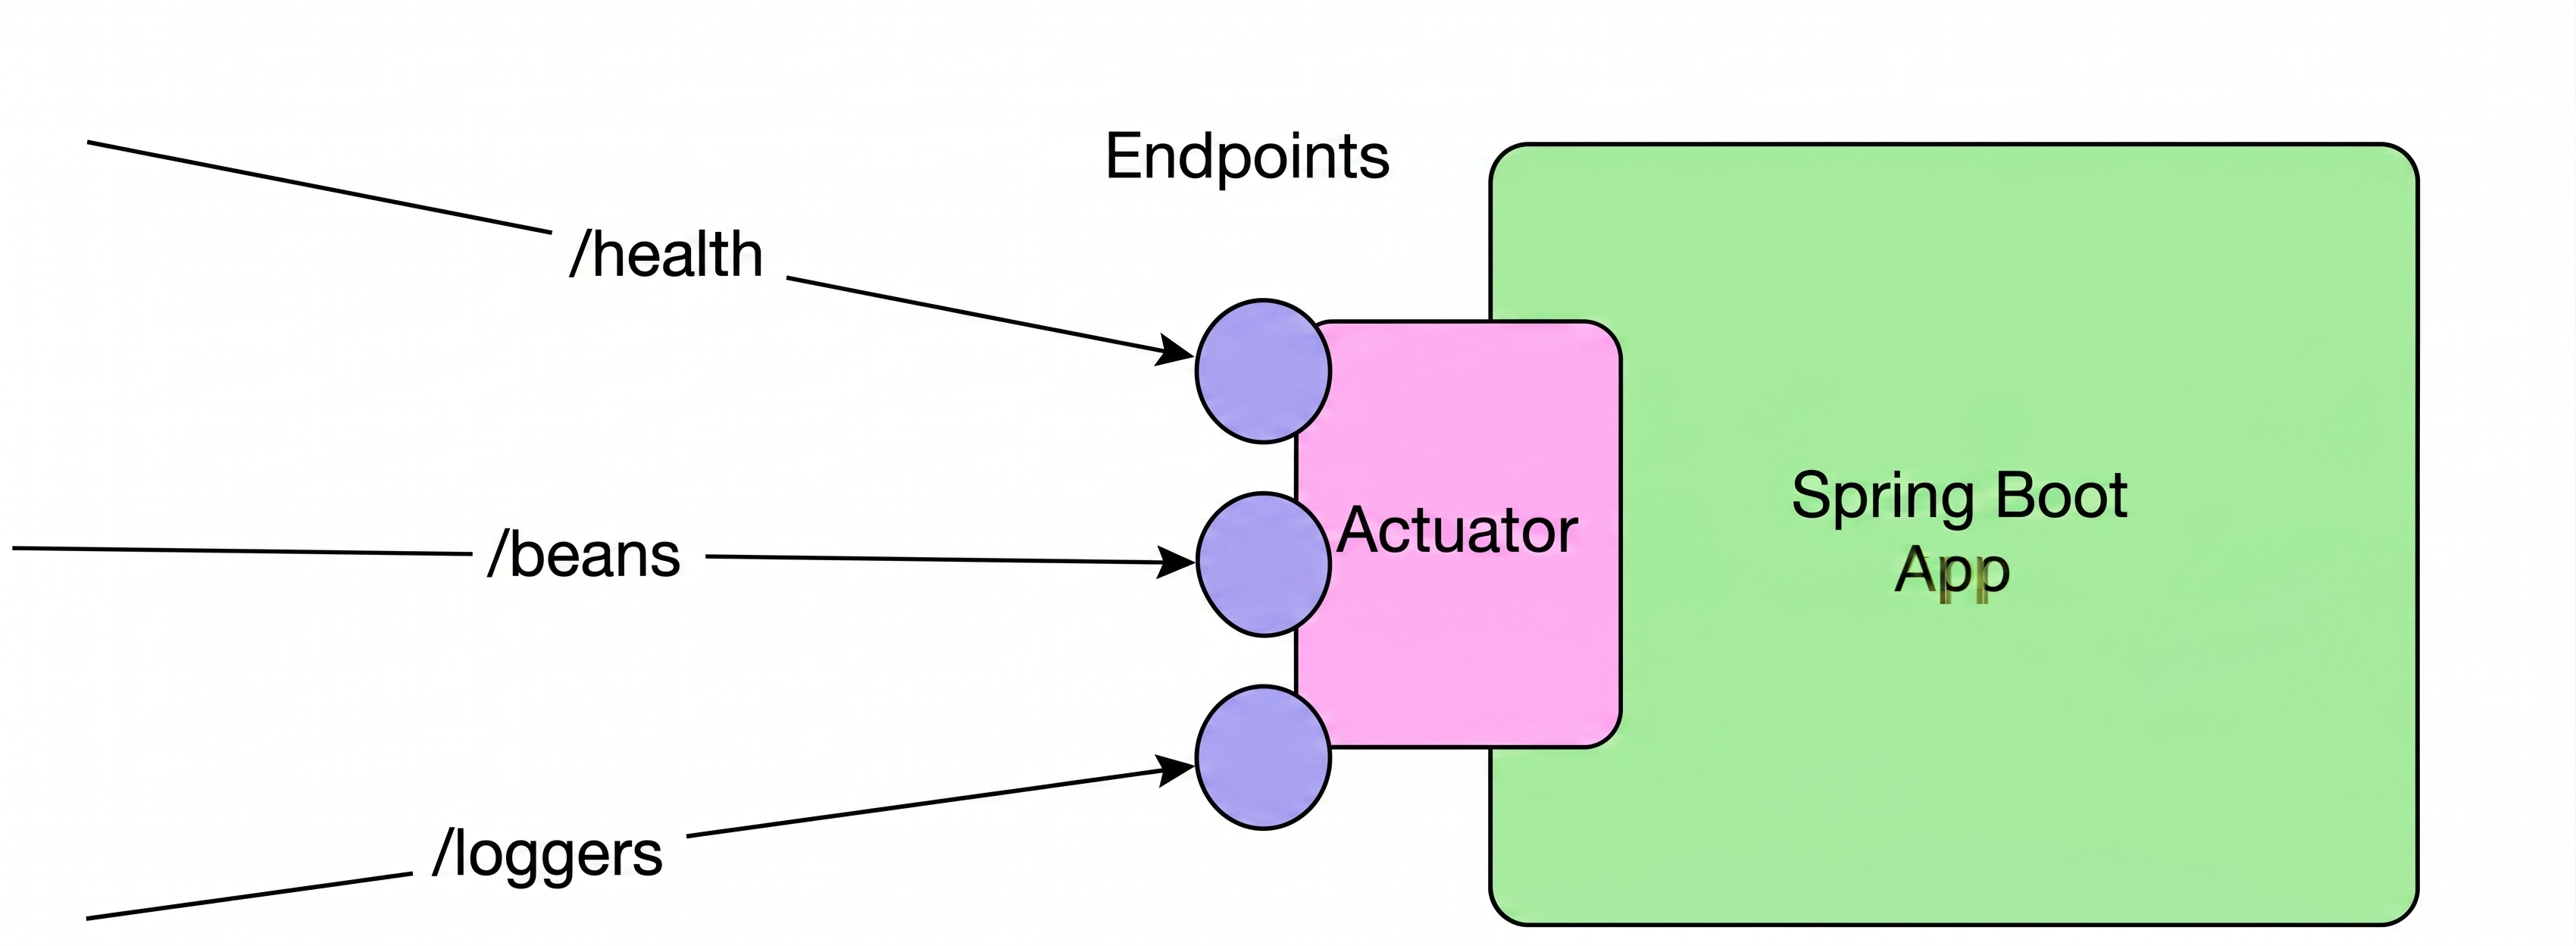
\includegraphics[width=0.8\textwidth]{imagenes/documento/actuador.png} 
    \caption{Visualización de los Endpoints de monitoreo proporcionados por Spring Boot Actuator.\cite{51}}
    \label{fig:spring_actuator_endpoints}
\end{figure}
% ------------------------------

Esta capacidad de inspección es fundamental para asegurar la integridad de la inversión de control, permitiendo verificar que componentes críticos como los repositorios de persistencia han sido correctamente instanciados \cite{51}.

\paragraph{Importancia en Entornos de Contenedores}
En arquitecturas modernas basadas en Docker y Kubernetes, Actuator facilita la implementación de pruebas de vida y disponibilidad (\textit{Liveness} y \textit{Readiness probes}), optimizando la disponibilidad del servicio mediante la gestión automatizada del orquestador.




\subsubsection{Spring Security (JWT y OAuth2)}

Spring Security proporciona un soporte integral para la implementación de servidores de recursos (\textit{Resource Servers}) bajo el estándar OAuth 2.0, utilizando tokens \textbf{JWT (JSON Web Tokens)} para la autorización de solicitudes \cite{52}. Este esquema permite que la aplicación valide de forma segura la identidad y los permisos del cliente mediante el uso de tokens portadores (\textit{Bearer Tokens}) sin necesidad de mantener sesiones en el servidor.

\paragraph{Dependencias Mínimas para JWT}
Para que un servidor de recursos sea funcional y capaz de decodificar y verificar firmas criptográficas, es necesaria la inclusión de dos bibliotecas fundamentales en el archivo \texttt{pom.xml} \cite{52}:
\begin{itemize}
    \item \texttt{spring-security-oauth2-resource-server}: Contiene el soporte base para la gestión de servidores de recursos.
    \item \texttt{spring-security-oauth2-jose}: Proporciona la infraestructura necesaria para el procesamiento de objetos \textit{Javascript Object Signing and Encryption} (JOSE), requerida para validar los JWT.
\end{itemize}

Al establecer esta propiedad, el sistema lanza un proceso de descubrimiento determinista que consulta los \textit{metadata endpoints} del proveedor para configurar las estrategias de validación de firmas y algoritmos de confianza (por defecto RS256) \cite{52}.

\paragraph{Arquitectura y Proceso de Autenticación}
El componente central es el \texttt{JwtAuthenticationProvider}, el cual utiliza un \texttt{JwtDecoder} para procesar el token y un \texttt{JwtAuthenticationConverter} para transformar los \textit{claims} del JSON en autoridades de seguridad \cite{52}.

\begin{figure}[htbp]
    \centering
    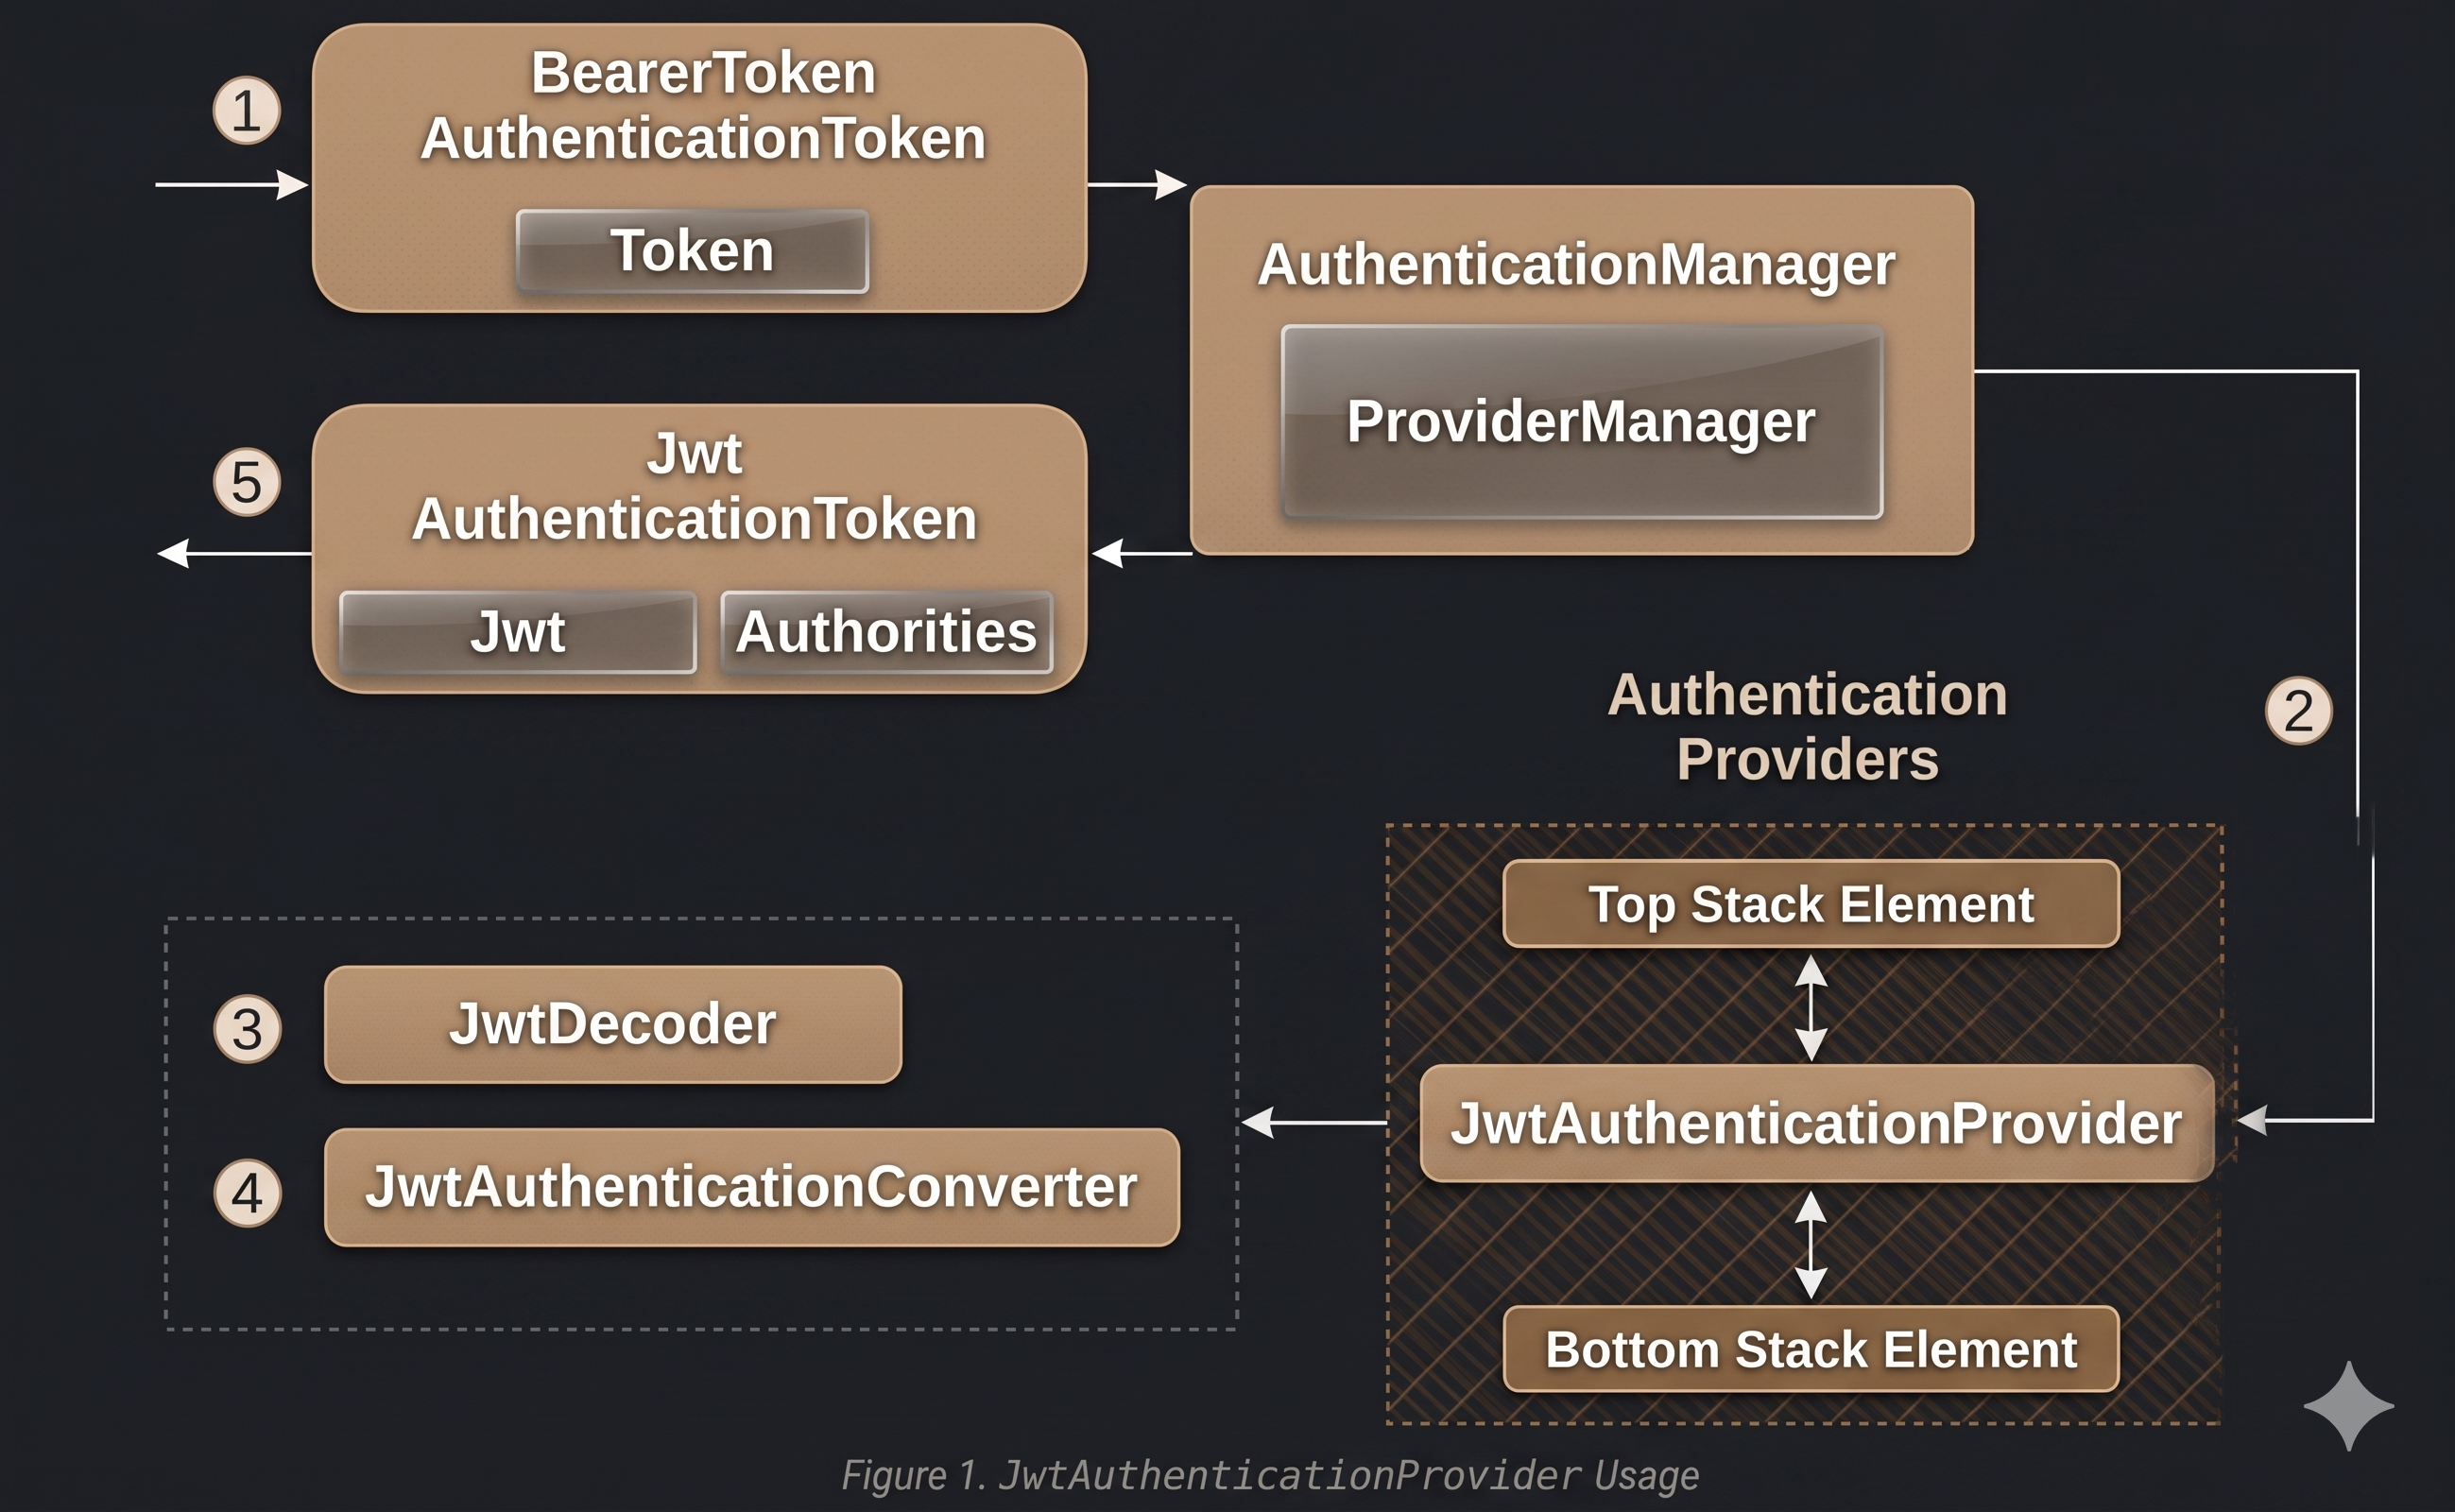
\includegraphics[width=0.9\textwidth]{imagenes/documento/jwtyauth2.png} 
    \caption{Uso de JwtAuthenticationProvider en el flujo de autenticación de Spring Security \cite{52}.}
    \label{fig:jwt_auth_flow}
\end{figure}

Una vez que el servidor de recursos recibe una petición con el encabezado \texttt{Authorization: Bearer}, se ejecutan las siguientes validaciones automáticas \cite{52}:
\begin{enumerate}
    \item \textbf{Firma:} Se verifica contra la llave pública obtenida del \texttt{jwks\_url}.
    \item \textbf{Vigencia:} Se validan las marcas de tiempo de expiración (\textit{exp}) y no antes de (\textit{nbf}).
    \item \textbf{Emisor:} Se confirma que el \textit{claim} \textit{iss} coincida con el configurado en la aplicación.
\end{enumerate}

\paragraph{Autorización Basada en Scopes}
Los tokens emitidos suelen incluir un atributo \texttt{scope} o \texttt{scp}. Spring Security mapea estos atributos prefijándolos con la cadena \texttt{SCOPE\_}, permitiendo restringir el acceso a rutas específicas mediante la cadena de filtros \cite{52}:

\begin{verbatim}
@Bean
public SecurityFilterChain filterChain(HttpSecurity http) throws Exception {
    http
        .authorizeHttpRequests((authorize) -> authorize
            .requestMatchers("/reportes/**").access(hasScope("reportes:lectura"))
            .anyRequest().authenticated()
        )
        .oauth2ResourceServer((oauth2) -> oauth2.jwt(Customizer.withDefaults()));
    return http.build();
}
\end{verbatim}

Este mecanismo garantiza que el sistema solo procese solicitudes de usuarios que posean los permisos exactos requeridos para interactuar con los expedientes de la Defensoría \cite{52}.

\subsubsection{Spring Cloud (Config Server y Eureka Service Discovery)}

En el desarrollo de arquitecturas distribuidas para la Defensoría de los Derechos Politécnicos, la gestión manual de configuraciones y la localización de servicios resulta ineficiente. Spring Cloud proporciona una serie de herramientas para resolver problemas comunes en sistemas distribuidos, tales como la gestión de configuraciones y el descubrimiento de servicios \cite{53}.

\paragraph{Spring Cloud Config Server}
Este componente actúa como un servidor centralizado para la gestión de configuraciones externas en un sistema distribuido. Sus características principales incluyen \cite{53}:
\begin{itemize}
    \item \textbf{Centralización:} Permite desacoplar las propiedades de configuración (como credenciales de bases de datos o parámetros del clasificador de IA) del código fuente, almacenándolas en un repositorio centralizado (generalmente Git) \cite{53}.
    \item \textbf{Gestión por Entornos:} Facilita el manejo de diferentes perfiles (desarrollo, pruebas y producción) de forma transparente para los microservicios \cite{53}.
    \item \textbf{Actualización Dinámica:} A través de anotaciones como \texttt{@RefreshScope}, el sistema puede actualizar parámetros en tiempo de ejecución sin necesidad de reiniciar las instancias de los servicios, garantizando la continuidad operativa \cite{53}.
\end{itemize}

\paragraph{Eureka Service Discovery}
Dada la naturaleza dinámica de los contenedores Docker en el entorno del proyecto, donde las direcciones IP pueden cambiar frecuentemente, se implementa Eureka como mecanismo de localización automática \cite{53}:
\begin{itemize}
    \item \textbf{Eureka Server:} Funciona como un directorio de servicios donde cada microservicio se registra al iniciar, informando su dirección de red y estado de salud \cite{53}.
    \item \textbf{Eureka Client:} Permite que los microservicios se localicen entre sí mediante nombres lógicos (ej. \texttt{servicio-ia-clasificador}) en lugar de direcciones IP estáticas, facilitando el balanceo de carga y la tolerancia a fallos \cite{53}.
    \item \textbf{Monitoreo de Estado:} El servidor Eureka utiliza un mecanismo de \textit{heartbeat} para detectar si una instancia ha caído, eliminándola automáticamente del registro para evitar errores de comunicación en el ecosistema \cite{53}.
\end{itemize}

Esta infraestructura asegura que el sistema sea escalable y mantenible, permitiendo una comunicación fluida entre el repositorio digital y el módulo de consulta ciudadana \cite{53}.


\subsection{Interfaces de Programación (API REST): Estándares de interoperabilidad, documentación y versionamiento}

Las interfaces de programación de aplicaciones bajo el estilo arquitectónico REST (\textit{Representational State Transfer}) constituyen el estándar de comunicación entre los microservicios del sistema y el \textit{front-end}. Este enfoque permite la interoperabilidad entre plataformas heterogéneas mediante el uso de protocolos estándar de la web \cite{54}.

\paragraph{Estándares de Interoperabilidad y HTTP/2}
Para garantizar una comunicación eficiente y escalable, el sistema se adhiere a los principios de REST, utilizando los verbos de transferencia HTTP (GET, POST, PUT, DELETE) para definir operaciones semánticas sobre los recursos. La implementación aprovecha las ventajas de \textbf{HTTP/2}, que introduce la multiplexación de peticiones y la compresión de cabeceras, reduciendo significativamente la latencia en la carga de expedientes y reportes dentro de la plataforma \cite{54}.

\paragraph{Estrategias de Versionamiento y Rate Limiting}
Dado que el sistema está sujeto a evoluciones normativas y técnicas, se implementan mecanismos de control para asegurar la compatibilidad:
\begin{itemize}
    \item \textbf{Versioning:} Se adopta el versionado a través de la URI (ej. \texttt{/v1/expedientes}), lo que permite coexistir diferentes versiones de un mismo servicio mientras se migran las funcionalidades \cite{54}.
    \item \textbf{Rate Limiting (Bucket4j):} Para proteger la integridad del repositorio digital ante posibles ataques de denegación de servicio o saturación, se implementa un control de tasa de peticiones. Esto asegura que el consumo de recursos se mantenga dentro de los límites operativos permitidos por la infraestructura \cite{54}.
\end{itemize}

Esta capa de servicios garantiza que la información de los derechos politécnicos sea accesible, segura y fácil de integrar con futuros módulos institucionales \cite{54}.

\section{Seguridad y Comunicación de Datos (En Tránsito)}

La seguridad de los datos en tránsito se refiere a las medidas de protección aplicadas a la información mientras esta se desplaza a través de una red, ya sea pública o privada. En una arquitectura de microservicios, asegurar el canal de comunicación es crítico para evitar ataques de intermediario (\textit{Man-in-the-Middle}) y garantizar la integridad de los expedientes de la Defensoría\cite{55}.

\subsection{Protocolos de Transporte Seguro: TLS 1.3}

Para cifrar las comunicaciones en la capa de transporte, el sistema implementa el protocolo \textbf{TLS (Transport Layer Security) 1.3}\cite{55}. Esta versión ofrece mejoras significativas sobre sus predecesores:
\begin{itemize}
    \item \textbf{Reducción de Latencia:} Optimiza el proceso de \textit{handshake}, permitiendo que la conexión se establezca más rápido, lo cual es vital para el rendimiento de los microservicios\cite{55}.
    \item \textbf{Seguridad Reforzada:} Elimina algoritmos criptográficos obsoletos y vulnerables, obligando al uso de técnicas modernas de cifrado autenticado\cite{55}.
    \item \textbf{Privacidad de Forwarding:} Garantiza que, incluso si una clave de sesión se ve comprometida en el futuro, las comunicaciones pasadas permanezcan cifradas\cite{55}.
\end{itemize}

\paragraph{Mecanismos de Seguridad Reforzada}
A diferencia de sus predecesores, TLS 1.3 elimina el soporte para algoritmos criptográficos considerados obsoletos o inseguros (como MD5, SHA-1 y suites de cifrado de exportación), obligando al uso exclusivo de técnicas modernas de cifrado autenticado basadas en \textbf{AEAD} (\textit{Authenticated Encryption with Associated Data}) \cite{1, 56}. Esto garantiza que cada paquete de información no solo esté cifrado, sino que su autenticidad sea verificada de forma simultánea, impidiendo ataques de manipulación de datos \cite{56}.

\paragraph{Optimización del Handshake y 0-RTT}
Una de las mejoras más significativas de TLS 1.3 es la reducción drástica en la latencia de conexión \cite{56}:
\begin{itemize}
    \item \textbf{Handshake de un solo viaje (1-RTT):} Reduce a la mitad el número de interacciones necesarias entre el cliente y el servidor para establecer una clave de cifrado común, en comparación con el proceso requerido en TLS 1.2 \cite{56}.
    \item \textbf{0-RTT (Zero Round Trip Time Resumption):} Permite que los usuarios que han establecido una conexión previa puedan enviar datos cifrados en el primer mensaje de la reconexión, acelerando la experiencia de usuario en el módulo de consulta ciudadana \cite{56}.
\end{itemize}

\paragraph{Perfect Forward Secrecy (PFS)}
Al hacer obligatorio el intercambio de claves mediante \textit{Ephemeral Diffie-Hellman}, TLS 1.3 asegura que, ante un hipotético compromiso de la clave privada del servidor en el futuro, las sesiones de comunicación capturadas en el pasado permanezcan cifradas e inaccesibles, proporcionando protección a largo plazo para los expedientes digitales \cite{56}.



Esta arquitectura híbrida asegura que los procesos pesados, como el análisis del clasificador neuro-simbólico, no degraden la respuesta del sistema frente al ciudadano \cite{57}.

\subsection{Resiliencia del Sistema: Patrones API Gateway (Spring Cloud Gateway) y Circuit Breaker (Resilience4j)}

En una arquitectura distribuida como la propuesta para la Defensoría de los Derechos Politécnicos, la resiliencia se define como la capacidad del sistema para recuperar su funcionamiento normal tras un fallo o para seguir operando ante errores parciales \cite{58}. Para evitar que un fallo en un microservicio sature los recursos de toda la infraestructura, se implementan patrones de diseño de alta disponibilidad \cite{58}.

\paragraph{API Gateway con Spring Cloud Gateway}
El patrón API Gateway actúa como un punto de entrada único y centralizado para todas las solicitudes de los clientes, gestionando la complejidad del ecosistema de microservicios de forma transparente \cite{58}. Sus funciones críticas incluyen:
\begin{itemize}
    \item \textbf{Enrutamiento Dinámico:} Dirige las peticiones entrantes hacia el microservicio correspondiente mediante la resolución de nombres proporcionada por Eureka \cite{58}.
    \item \textbf{Seguridad Perimetral:} Centraliza la validación de tokens JWT y la aplicación de políticas de seguridad antes de que la petición alcance los servicios internos \cite{58}.
    \item \textbf{Abstracción de Red:} Permite que el \textit{front-end} interactúe con un único dominio, ocultando la topología de la red interna y simplificando el manejo de CORS (\textit{Cross-Origin Resource Sharing}) \cite{58}.
\end{itemize}

\paragraph{Patrón Circuit Breaker mediante Resilience4j}
El patrón de interruptor o \textit{Circuit Breaker} es fundamental para prevenir fallos en cascada dentro del sistema \cite{58}. Utilizando la librería \textbf{Resilience4j}, el sistema monitoriza las llamadas a servicios externos (como el repositorio digital o el clasificador de IA) y gestiona su estado de la siguiente manera \cite{58}:
\begin{itemize}
    \item \textbf{Estado Cerrado (Closed):} El flujo de peticiones es normal. El interruptor contabiliza los éxitos y fallos de las operaciones de red \cite{58}.
    \item \textbf{Estado Abierto (Open):} Si el umbral de fallos se supera (debido a tiempos de espera agotados o errores de servidor), el interruptor se abre. En este estado, todas las peticiones fallan de inmediato, protegiendo los recursos de la infraestructura \cite{58}.
    \item \textbf{Estado Entreabierto (Half-Open):} Tras un periodo de espera, se permite el paso de un número limitado de peticiones de prueba para verificar si el servicio remoto se ha recuperado antes de volver al estado cerrado \cite{58}.
\end{itemize}

\paragraph{Estrategias de Fallback}
Complementando al \textit{Circuit Breaker}, se definen métodos de \textit{fallback} que proporcionan una respuesta alternativa predeterminada cuando un servicio no está disponible \cite{58}. Esto asegura que el ciudadano siempre reciba una respuesta informativa o una versión simplificada del servicio en lugar de un error crítico del sistema, manteniendo la confianza en la plataforma institucional \cite{58}.

\section{Infraestructura y Orquestación}

La infraestructura moderna para el despliegue de microservicios se fundamenta en la abstracción del hardware y la automatización del entorno de ejecución. Para el sistema de la Defensoría, se adopta un enfoque basado en contenedores, lo que garantiza que la aplicación se comporte de manera idéntica desde el entorno de desarrollo local hasta el servidor de producción en Hostinger \cite{58}.

\subsection{Contenerización: Fundamentos de Docker, Dockerfile y gestión con Docker Compose}

Docker es la plataforma de virtualización a nivel de sistema operativo que permite empaquetar software en unidades estandarizadas llamadas contenedores \cite{58}. Esta tecnología es crítica para asegurar la portabilidad del repositorio digital y sus microservicios \cite{58}.

\paragraph{Componentes y Definición}
El proceso de contenerización se rige por los siguientes elementos técnicos \cite{58}:
\begin{itemize}
    \item \textbf{Dockerfile:} Es un archivo de configuración basado en texto que contiene todas las instrucciones necesarias para construir una imagen de Docker \cite{58}. En este proyecto, se utiliza para definir el entorno de ejecución de Java, copiar los archivos JAR generados por Maven y configurar las variables de entorno necesarias \cite{58}.
    \item \textbf{Imágenes y Contenedores:} Una imagen es una plantilla de solo lectura que incluye el código, las librerías y las dependencias \cite{58}. El contenedor es la instancia ejecutable de dicha imagen, operando de forma aislada para evitar conflictos de librerías en el servidor \cite{58}.
    \item \textbf{Docker Compose:} Es una herramienta para definir y ejecutar aplicaciones Docker de múltiples contenedores \cite{58}. Mediante un archivo \texttt{docker-compose.yml}, se orquestan servicios como la base de datos PostgreSQL, el servidor Eureka y los microservicios de Spring Boot, permitiendo levantar toda la infraestructura con un único comando \cite{58}.
\end{itemize}

\subsection{Orquestación de Contenedores: Kubernetes (K8s), gestión de Pods, Deployments y escalabilidad horizontal (HPA)}

Kubernetes es una plataforma de código abierto diseñada para automatizar el despliegue, el escalado y la gestión de aplicaciones contenerizadas \cite{59}. En este Trabajo Terminal, K8s proporciona la capa de orquestación necesaria para garantizar la alta disponibilidad \cite{59}.

\paragraph{Abstracciones de Kubernetes}
El sistema se organiza mediante los siguientes objetos de orquestación \cite{59}:
\begin{itemize}
    \item \textbf{Pods:} Es la unidad mínima de ejecución en Kubernetes \cite{59}. Un Pod agrupa uno o más contenedores (como el microservicio de Java) que comparten almacenamiento y red, actuando como una única entidad lógica dentro del clúster \cite{59}.
    \item \textbf{Deployments:} Describen el estado deseado de los Pods \cite{59}. El controlador de Deployment se encarga de cambiar el estado actual al deseado a una tasa controlada, permitiendo actualizaciones sin tiempo de inactividad (\textit{rolling updates}) y recuperaciones automáticas ante fallos \cite{59}.
    \item \textbf{Horizontal Pod Autoscaler (HPA):} Es el mecanismo encargado de la escalabilidad horizontal \cite{59}. El HPA escala automáticamente el número de Pods en un Deployment basándose en métricas de utilización de CPU o memoria \cite{59}. Por ejemplo, si el clasificador neuro-simbólico detecta una carga inusual durante el procesamiento de quejas, el HPA instanciará nuevos Pods para distribuir la carga y mantener la respuesta del sistema \cite{59}.
\end{itemize}

Esta infraestructura de orquestación asegura que la plataforma de la Defensoría sea resiliente y capaz de adaptarse a la demanda de los usuarios de manera autónoma \cite{59}.

\section{Gestión de Bases de Datos}

\subsection{PostgreSQL}

PostgreSQL es un sistema de gestión de bases de datos relacionales de objetos (ORDBMS) de código abierto, reconocido por su fiabilidad, robustez de funciones y rendimiento, lo que permite gestionar cargas de trabajo de datos complejas de forma segura \cite{42}.

\textbf{Ventajas de su uso:}
\begin{itemize}
\item \textbf{Integridad y Seguridad de Datos:} Cumple estrictamente con el modelo ACID, garantizando que todas las transacciones se procesen de forma fiable \cite{42}.
\item \textbf{Extensibilidad y Versatilidad:} Permite definir tipos de datos personalizados y soporta diversos lenguajes \cite{42}.
\item \textbf{Soporte y Estándares:} Su alta adherencia a SQL asegura la compatibilidad con múltiples herramientas de análisis \cite{42}.
\end{itemize}

\section{Persistencia y Gestión del Repositorio Digital (En Reposo)}

La persistencia de la información en el sistema de la Defensoría se fundamenta en el uso de bases de datos relacionales de objetos de alto rendimiento. Se define como datos "en reposo" a toda la información que se encuentra almacenada de forma persistente en soportes físicos, requiriendo mecanismos específicos de integridad y seguridad para su preservación a largo plazo \cite{60}. El repositorio digital no solo actúa como un almacén, sino como un sistema de gestión de activos digitales que garantiza la disponibilidad y la inmutabilidad de los expedientes jurídicos \cite{60}.

\subsection{PostgreSQL Avanzado: Manejo de datos semi-estructurados (JSONB) e indexación GIN para búsqueda de texto completo (Full-text search)}

PostgreSQL se ha consolidado como la opción preferida para el repositorio digital debido a su arquitectura extensible y su capacidad para manejar esquemas híbridos que combinan el rigor relacional con la flexibilidad documental \cite{60}.

\paragraph{Manejo de JSONB y Modelado NoSQL}
A diferencia del tipo de datos JSON estándar, que almacena una copia exacta del texto, el formato \textbf{JSONB} (\textit{JSON Binary}) almacena los datos en un formato binario descompuesto \cite{60}. Esta implementación permite:
\begin{itemize}
    \item \textbf{Optimización del Rendimiento:} Aunque la inserción conlleva un costo computacional adicional debido al procesamiento binario, el análisis y la recuperación son significativamente más veloces, ya que se evita el re-parseo del texto en cada consulta \cite{60}.
    \item \textbf{Evolución del Esquema:} Facilita el almacenamiento de metadatos variables de los expedientes, tales como anexos técnicos o formularios dinámicos, que no se ajustan a una estructura tabular rígida, sin comprometer la capacidad de realizar consultas complejas \cite{60}.
    \item \textbf{Operadores de Contención:} Permite el uso de operadores especializados (como \texttt{@>}) para verificar si un documento JSONB contiene ciertos pares clave-valor de forma eficiente \cite{60}.
\end{itemize}

\paragraph{Búsqueda de Texto Completo e Índices GIN}
Para la recuperación eficiente de información dentro del cuerpo de los documentos legales y quejas, se implementa \textit{Full-Text Search} mediante \cite{60}:
\begin{itemize}
    \item \textbf{Componentes Lingüísticos (tsvector y tsquery):} Los documentos se procesan mediante diccionarios para eliminar \textit{stop-words} y realizar \textit{stemming} (reducción a la raíz), transformándolos en vectores de lexemas que permiten búsquedas semánticas y no solo literales \cite{60}.
    \item \textbf{Índices GIN (Generalized Inverted Index):} Este tipo de indexación es fundamental para el manejo de JSONB y búsqueda de texto, ya que funciona como un índice invertido que mapea cada término o clave a la lista de registros que lo contienen, acelerando exponencialmente las consultas sobre los grandes volúmenes de datos que genera la Defensoría \cite{60}.
\end{itemize}

\subsection{Seguridad y Cifrado en Reposo: Implementación de pgcrypto (AES-256) y validación de integridad mediante hashes SHA-512}

La protección de los datos en reposo es una exigencia legal estricta bajo la LFPDPPP para salvaguardar la privacidad de los miembros de la comunidad politécnica \cite{60}. Se utiliza la extensión \textbf{pgcrypto} para implementar criptografía robusta a nivel de motor de base de datos \cite{60}.

\paragraph{Cifrado Simétrico con AES-256}
Se utiliza el estándar \textbf{AES (Advanced Encryption Standard)} con llaves de 256 bits en modo CBC o GCM para cifrar campos sensibles como nombres de involucrados, folios internos y descripciones detalladas de vulneraciones de derechos \cite{60}. Este mecanismo asegura que, ante una extracción no autorizada de los archivos físicos de la base de datos (\textit{tablespaces}), la información permanezca cifrada e inaccesible sin la llave maestra protegida por políticas de acceso estrictas \cite{60}.

\paragraph{Integridad Estricta con Hashes SHA-512}
Para garantizar que un expediente no ha sido alterado accidental o malintencionadamente, se implementa una estrategia de \textit{hash-chaining} o sellado digital \cite{60}. Se genera un compendio único utilizando el algoritmo \textbf{SHA-512}, el cual es altamente resistente a colisiones \cite{60}. Cualquier modificación mínima en el registro dispararía una discrepancia en el hash, permitiendo auditorías de integridad inmediatas sobre el repositorio \cite{60}.

\subsection{Escalabilidad de Base de Datos: Particionamiento de tablas, pooling de conexiones (PgBouncer) y replicación streaming}

La arquitectura del repositorio digital debe contemplar un crecimiento sostenido de la información, aplicando estrategias que optimicen el uso de recursos en el servidor VPS \cite{60}.

\begin{itemize}
    \item \textbf{Particionamiento por Rango (Table Partitioning):} Se segmentan las tablas de expedientes por periodos anuales o semestrales. Esto mejora el rendimiento de las consultas al realizar un \textit{partition pruning}, donde el motor de búsqueda ignora las particiones que no contienen el rango de fechas solicitado, reduciendo drásticamente las operaciones de E/S en disco \cite{60}.
    \item \textbf{Pooling de Conexiones con PgBouncer:} Dado que los microservicios de Spring Boot operan de forma concurrente, PgBouncer gestiona una cola de conexiones hacia PostgreSQL \cite{60}. Esto evita el consumo excesivo de memoria RAM que implicaría crear un nuevo proceso por cada solicitud, manteniendo la estabilidad del servidor ante picos de tráfico en el módulo ciudadano \cite{60}.
    \item \textbf{Replicación Streaming y Alta Disponibilidad:} Se configura una réplica en modo \textit{Hot Standby}, permitiendo que un servidor secundario reciba de forma continua los registros de transacciones (WAL). Esta técnica no solo sirve como respaldo ante desastres, sino que permite descargar las operaciones de consulta (lectura) del servidor principal para balancear la carga de trabajo \cite{60}.
\end{itemize}

